\chapter{Advisor}\label{chapter:advisor}

To enable performance-aware and constraint-driven migration between \acrshort{orm} frameworks, the proposed approach incorporates a dedicated optimization component, referred to as the \emph{advisor}. This module is responsible for selecting the most suitable \acrshort{orm} framework -- or a combination thereof -- for executing a given query workload while adhering to user-specified constraints, such as memory limits or framework usage caps. Although syntactic translation guarantees semantic preservation, optimal runtime performance and memory efficiency require deliberate framework selection grounded in empirical metrics and formal optimization.

This framework selection task is formulated as an instance of \emph{Integer Linear Programming} (\acrshort{ilp}), allowing the selection process to be guided by a quantitative model that balances execution time, memory usage, and user-defined bounds. This approach transforms what would otherwise be a trial-and-error or heuristic-based process into a mathematically grounded, reproducible method that yields optimal, or probably near-optimal, results. The \acrshort{ilp} instance is solved using an embedded solver, specifically the open-source GNU Linear Programming Kit (\acrshort{glpk}),\footnote{\url{https://www.gnu.org/software/glpk/}} which supports binary and mixed-integer optimization through its branch-and-bound implementation.

\section{What-if analysis}

Before invoking the \acrshort{ilp} solver, a comprehensive \emph{what-if analysis} is conducted to gather the performance data required for optimization. This phase evaluates each input query across a set of \acrshort{orm} frameworks, including both the original source framework and selected targets. For every query-framework pair, the system first performs a syntactic translation of the query into the appropriate framework representation. The resulting queries are then executed against a common underlying database system to measure empirical performance.

Let $W $ denote the set of all input queries and $F$ the set of \acrshort{orm} frameworks under evaluation. Each query $q \in W$ is executed under each framework $f \in F$, producing two primary performance metrics:
\begin{itemize}
    \item \textit{Runtime}, in milliseconds, representing query execution latency.
    \item \textit{Memory footprint}, in kilobytes, capturing the peak memory used during query execution.
\end{itemize}

%Each query $q$ is also assigned a frequency weight $z_q$, representing its relative importance within the workload. This allows the \acrshort{ilp} objective function to emphasize performance on frequently executed queries.

The result of the analysis is a set of matrices -- $\text{cost}(q,f)$ for runtime and $\text{mem}(q,f)$ for memory usage, where $q \in W$, $f \in F$. %The user can specify:
% \begin{itemize}
%     \item A total memory constraint $\text{MEM} \in \mathbb{R}_{>0}$,
%     \item A limit on the number of frameworks $N \in \mathbb{N}$.
% \end{itemize}

\section{ILP formulation}

Formally, let $W$ be the set of queries and $F$ the set of ORM frameworks. For each query $q \in W$, its relative importance is captured by a frequency parameter $z_q$. Empirical measurements yield $\text{cost}(q, f)$, the runtime of query $q$ on framework $f$, and $\text{mem}(q, f)$, the corresponding memory usage. The global memory constraint is denoted $\text{MEM} \in \mathbb{R}_{>0}$, and the upper bound on the number of frameworks to be used is given by $N \in \mathbb{N}$. Decision variables $x_{q,f} \in \{0,1\}$ indicate whether query $q$ is assigned to framework $f$, and $y_f \in \{0,1\}$ indicates whether framework $f$ is selected.

The optimization objective is to minimize the total weighted cost:
$$\min \sum_{q \in W} \sum_{f \in F} z_q \cdot \text{cost}(q, f) \cdot x_{q,f}$$

\noindent
subject to the following constraints:
\begin{align}
&\sum_{f \in F} y_f \leq N && \tag{1} \\
&\sum_{f \in F} x_{q,f} = 1 && \forall q \in W \quad \tag{2} \\
&x_{q,f} \leq y_f && \forall q \in W,\ \forall f \in F \quad \tag{3} \\
&\sum_{q \in W} \sum_{f \in F} \text{mem}(q,f) \cdot x_{q,f} \leq \text{MEM} && \tag{4}
\end{align}

These constraints ensure that (1) no more than $N$ frameworks are selected, (2) each query uses one framework, (3) each query uses only selected frameworks, and (4) the total memory usage remains within the allowed budget.

The resulting \acrshort{ilp} instance is solved using an off-the-shelf solver such as \emph{Gurobi}\footnote{\url{https://www.gurobi.com}} or, in this particular case, \acrshort{glpk}, which searches the feasible solution space and returns an assignment of queries to frameworks that minimizes the objective while satisfying all constraints.

\section{Implementation using GLPK}

This \acrshort{ilp} model is implemented using the \acrshort{glpk} C \acrshort{api}. The optimization model is created using:

\begin{itemize}
    \item \texttt{glp\_create\_prob()} -- to initialize the problem instance.
    \item \texttt{glp\_add\_cols()}, \texttt{glp\_set\_col\_kind()} -- to define binary variables $x_{q,f}$ and $y_f$.
    \item \texttt{glp\_set\_obj\_coef()} -- to define the cost-weighted objective function.
    \item \texttt{glp\_add\_rows()} and \texttt{glp\_set\_row\_bnds()} -- to define constraints.
    \item \texttt{glp\_load\_matrix()} -- to load the sparse matrix of coefficients.
\end{itemize}

The solver is then executed via:
\begin{itemize}
    \item \texttt{glp\_init\_iocp()} -- to set solver parameters.
    \item \texttt{glp\_intopt()} -- to solve the \acrshort{ilp} using branch-and-bound.
\end{itemize}

Note that post-processing reads back the optimized variable values utilizing function \texttt{glp\_mip\_col\_val()}.

The \acrshort{ilp} constraints are mapped directly as rows in \acrshort{glpk}:

\begin{itemize}
    \item One row for the framework count: $\sum_f y_f \leq N$,
    \item One row per query to ensure assignment to one framework,
    \item $|W| \cdot |F|$ rows enforcing $x_{q,f} \leq y_f$,
    \item A final row aggregating memory usage across all $x_{q,f}$.
\end{itemize}

All variables are declared binary.

% \begin{figure}
% \centering
% 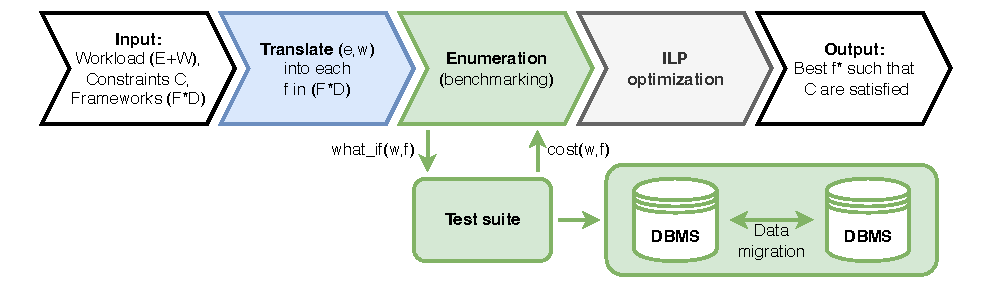
\includegraphics[scale=0.8]{thesis/img/thesis/ORM-workflow.pdf}
% \caption{TODO: Workflow }
% \label{fig:workflow}
% \end{figure}

%\afterpage{
%\begin{landscape}
\begin{figure}[!htp]
\centering
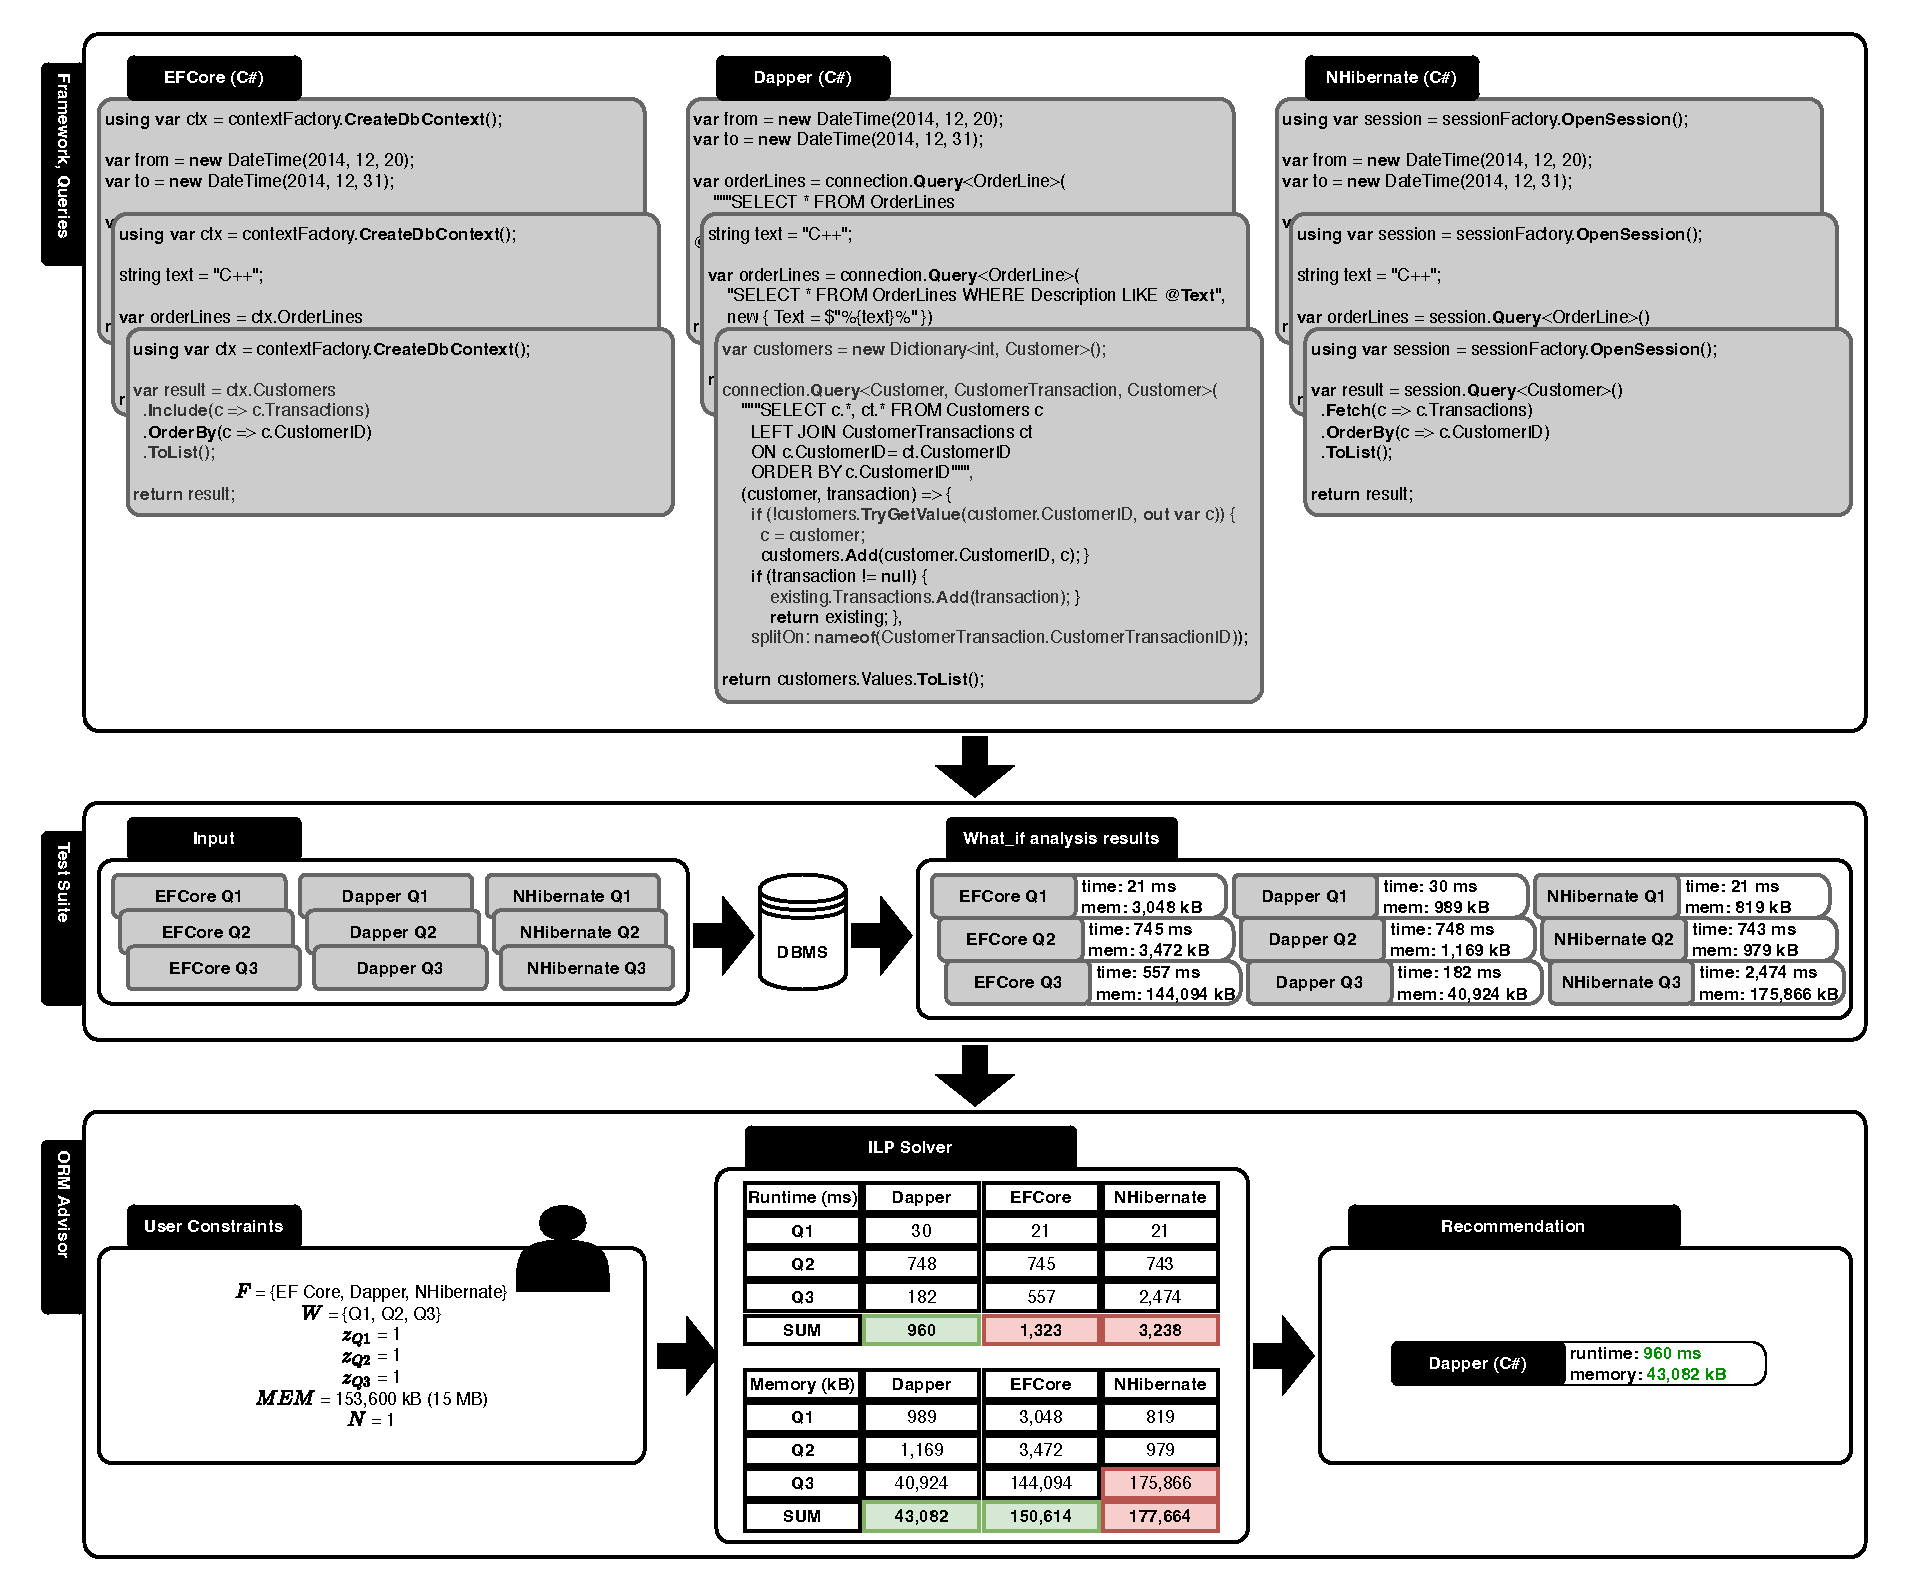
\includegraphics[width=\textwidth]{thesis/img/thesis/ORM-example.pdf}
\caption{An example of recommendation of optimal \acrshort{orm} framework}
\label{fig:example}
\end{figure}    
%\end{landscape}
%}

\begin{example}    
\small
Figure~\ref{fig:example} illustrates the optimization workflow supported by the advisor. In this scenario, it is assumed that the translation of queries and entity mappings from the input \acrshort{orm} framework (i.e., \acrshort{ef} Core) into the representations required by the selected target frameworks (i.e., Dapper, and NHibernate) has already been completed. Together with user-defined constraints, such as query weights, the maximum number of frameworks (e.g., $N = 1$ and an overall memory usage limit (e.g., $\text{mem} = 153,600$ kB), these artifacts form the input.

The process begins with a what-if analysis, where test suite is utilized to execute each framework-query pair against a shared database system. This benchmarking phase collects empirical performance data for each pair, specifically measuring average execution time and peak memory consumption.

The advisor then passes the collected performance metrics, along with the user-specified constraints, to the \acrshort{ilp} solver. The solver computes an optimal assignment of queries to frameworks that minimizes the total weighted runtime while adhering to all specified limitations. In this example, the recommended configuration assigns all queries to Dapper, as it achieves the best overall performance within the given constraints.
\qed
\end{example}

\section{Extensions beyond framework selection}
\label{sec:advisor_extensions}

While the advisor focuses on selecting the optimal \acrshort{orm} framework under performance and resource constraints, the underlying \acrshort{ilp} formulation provides a flexible foundation that can be extended to address broader data management strategies. One significant extension could be the incorporation of multiple database systems as part of the optimization space. In such extended model, the set of alternatives expands from frameworks alone to combinations of \acrshort{orm} frameworks and database backends, such as PostgreSQL, MySQL, or \acrshort{nosql} variants like MongoDB. Each pairing may exhibit different runtime and memory characteristics, and these empirical costs can be included in the what-if analysis.

Another possible extension involves modelling data redundancy and replication strategies. Rather than assigning each query to a single logical representation, queries may be routed to replicated or denormalized data stores optimized for specific access patterns. The \acrshort{ilp} model can include variables indicating which queries are permitted to use redundant copies and which entities are replicated across systems. Additional constraints can enforce storage budgets, consistency preferences, or replication limits.
